\chapter{Line Properties}

\section{Introduction}
\label{s:introduction}
Curvilinear structures are important in many applications of computer vision, including aerial image analysis (roads, rivers, railways), fingerprint analysis (ridges) and medical image analysis (blood vessels, ducts). As a result, there is an extensive literature on detecting such structure~\cite{Papari_Petkov_IVC11}. The literature on estimating the local orientation of curvilinear structure is more limited though the problem is equally important, for example as a basis for non-maximal suppression (centre-line detection) and for characterising properties such as tortuosity (\eg~of blood vessels).

In mammography, malignant lesions often exhibit linear structures (known as spicules) that form a radial pattern around the central mass. Detecting linear structures and determining their orientation~\cite{Zwiggelaar_etal_MIA99,Zwiggelaar_etal_TMI04} can therefore indicate points where they converge and thus whether a mass or architectural distortion is present~\cite{Karssemeijer_teBrake_TMI96,Rangayyan_Ayres_MBEC06}. In other medical applications such as retinography (\fref{f:retinography}), the rate of change of orientation (\ie~tortuosity) of blood vessels can serve as a diagnostic indicator of vascular disease~\cite{Hart_etal_IJMI99}; though studies have shown that vessels can be detected and segmented~\cite{Staal_etal_TMI04,Ricci_Perfetti_TMI07,Dabbah_etal_MICCAI10}, few have addressed the problem of measuring their orientation and quantifying tortuosity.

Similarly, automatic fingerprint analysis typically begins by computing the orientation at each pixel via gradient-based filtering, often followed by some smoothing over a local patch~\cite{Bazen_Gerez_TPAMI02,Mei_etal_IVC09}. This orientation field is often parameterized -- via `phase portraits'~\cite{Li_etal_PR06} or polynomial approximation~\cite{Gu_etal_PR04}, for example -- to capture and interpret the underlying properties of the fingerprint such as its `singular points' where the orientation is no longer defined (\eg~at a delta or the centre of a whorl). Though smoothing orientation estimates at a local patch have been the subject of several investigations~\cite{Kass_Witkin_CVGIP87,Rao_Jain_TPAMI92,Perona_TIP98}, we deal only with the initial step of estimating orientation at every pixel.

In this paper we revisit the problem of orientation estimation, reviewing the basic theory, extending the state-of-the-art, and providing the results of extensive evaluation using both real and realistic synthetic images. The first step in estimating orientation usually involves applying a set of linear filters to the image, generally at multiple scales and orientations. As we will show later, the choice of filter-bank has a significant influence on both computational efficiency, and estimation accuracy. Our contribution is to explore the similarities and differences between different approaches, and provide empirical evidence of which work best in practice.

Given a set of filter-bank outputs, the second step in estimating orientation is to combine them in some way. There are two basic approaches: to find the scale at which the total magnitude of response is greatest, and combine the different filter responses at that scale analytically~\cite{Karssemeijer_teBrake_TMI96,Mei_etal_IVC09}; or to use a regression learning approach to combine the filter responses across all scales and orientations~\cite{Berks_etal_IPMI11}. Our contribution is to explore the technical details of orientation regression and provide a comprehensive evaluation of different combinations of filter-bank and analytic/regression methods. Overall we show that an approach based on combining dual-tree complex wavelet filtering with random forest regression achieves significantly better results than any of the other state-of-the-art approaches tested.

\begin{figure}[t]
\centering
\begin{tabular}{c c c}
\includegraphics[width=0.3\columnwidth]{\figpath/retina/02_test} &
\includegraphics[width=0.3\columnwidth]{\figpath/retina/02_manual1} &
\includegraphics[width=0.3\columnwidth]{\figpath/retina/002_orientation_masked} \\
%\includegraphics[height=0.15\textheight]{\figpath/retina/002_abs_error} \\
(a) & (b) & (c) \\
\end{tabular}
%
\caption{Estimating orientation in retinography: %
(a) input image; %
(b) ground truth mask indicating pixels belonging to a vessel; %
(c) orientation (indicated by colour) estimated using linear regression over \dtcwt~features. The mask was not used to estimate orientation. %
%(c) magnitude of error (note the regions of high error at points of bifurcation.)
}
\label{f:retinography}
\end{figure}




\section{Estimating Orientation via Machine Learning}
\label{s:learning}


\section{Experiments}
\label{s:expts}
In our first set of experiments, we present a quantitative evaluation of the three regressors on real retinography images and mammogram-like data for which we have ground truth. We also present qualitative results on some real mammography images and fingerprint images for which ground truth was not available.


\subsection{Real Retinographic Images}
\label{s:expts_retinography}
The publicly available DRIVE dataset~\cite{Staal_etal_TMI04} contains 40 full colour retinogram images (\fref{f:retinography}a) of $565{\times}584$ pixels, split into training (images 21-40) and test (images 01-20) sets. A hand-labelled mask that indicates vessel pixels (\fref{f:retinography}b) is also available for every image, enabling us to skeletonize the mask and approximate ground truth, $\theta_{gt}$, from the skeleton for every labelled pixel.\comment{It is questionable how well this constitutes ground truth}

For training, we first transform all images to monochrome via a weighted sum of the three RGB channels (though using only the green channel is also popular). We then selected 200\,000 vessel pixels randomly over the training set and computed filter responses to the second derivative filters (\fref{f:filters}e-f), Haar-like filters (\fref{f:filters}g-h) and the \dtcwt~for every selected pixel. We used the resulting 200\,000 feature vectors and their corresponding target orientations to train each of the three regressors.

During testing, we applied each regressor in turn to estimate the orientation, $\theta_{est}$, at every pixel for every test image and computed the orientation error with respect to ground truth,
%
\begin{equation}
	\theta_{err} = \frac{\angle(2\theta_{est}-2\theta_{gt})}{2}
\end{equation}

\noindent only at labelled vessel pixels in the test image mask (\fref{f:retinography}c).\comment{A reviewer will probably complain that this is cheating and that we should have used a classifier}

\begin{table}[b]
\centering
\begin{tabular}{l|c c c c}
							& \multicolumn{4}{c}{Feature Type} \\
							& Monogenic		& 2nd deriv.	& Haar				& \dtcwt \\
\hline
\input{retinogram_table.txt}
\end{tabular}
%
\caption{Median absolute error (degrees) for combinations of input feature and regressor on the DRIVE database of retinal images (images 01-20).}
\label{t:retinopathy}
\end{table}

\begin{figure}
\centering
\begin{tabular}{c c}
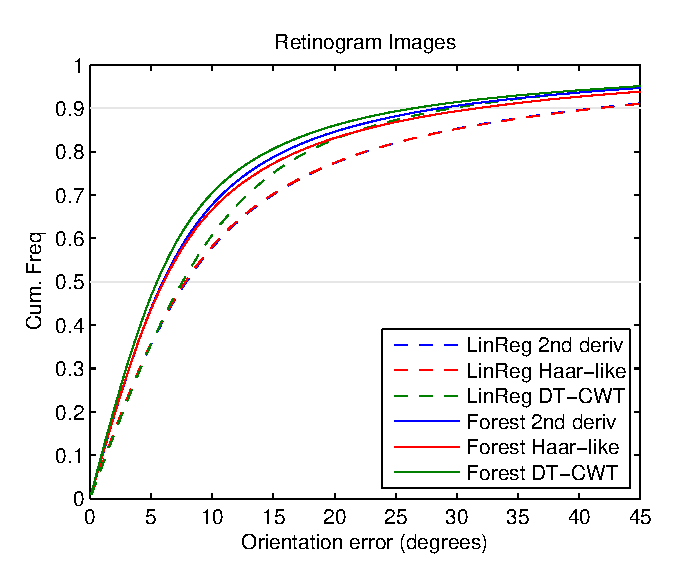
\includegraphics[width=0.48\columnwidth]{\figpath/retina/retinogram_expt} &
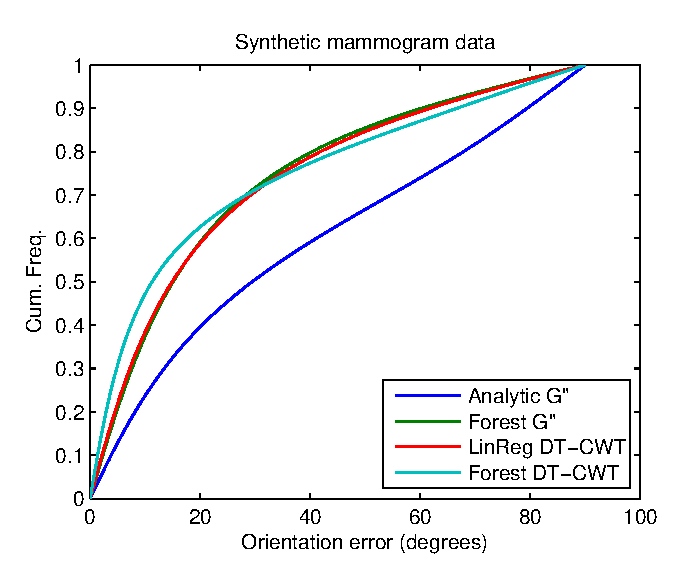
\includegraphics[width=0.48\columnwidth]{\figpath/mammo/mammography_expt} \\
(a) & (b) \\
\end{tabular}
%
\caption{Cumulative frequency of angular error for (a) retinogram images and (b) synthetic mammogram-like images.}
\label{f:cumfreq}
\end{figure}

Comparing performance for the various combinations (\fref{f:cumfreq}a and \tref{t:retinopathy}), we see that in general the analytic methods perform poorly in comparison with the regression approaches, that Random Forests outperform other regression methods and that the \dtcwt~is superior to other feature representations. With the exception of the boosted regressor, the Haar-like approximation exhibited similar performance to the second derivative, suggesting that it may be used effectively in scenarios where efficiency is a concern.

It may be surprising just how poorly the analytic formulations perform in contrast to the regressors. On inspection of the outputs, we see that the monogenic signal (based on first derivatives) does indeed fail at the centre of linear structures. Since, however, many of the vessels in the retinograms are a single pixel in width (such that anywhere on the line is at the centre by definition) the monogenic signal is doomed. The regressors also get some benefit from pooling responses over several pixels.

As noted earlier, when using squared or second derivative responses it is necessary to compute the responses at the two possible solutions to determine which is the correct one. With the Haar-like approximation that combines the response to $\Ixx$ and $\Iyy$, this analytic solution is not available and a regression approach becomes necessary. Also, since the linear regressor minimizes the average error it contains no mechanism for selecting the correct orientation in this way. This is likely to be one reason for its poor performance relative to more sophisticated regressors such as the Random Forest. There is a penalty, however, in efficiency when using complex regressors like the Random Forest.


\subsection{Mammogram-like Images}
\label{s:expts_synth_mammography}
\begin{table}[t]
\centering
\begin{tabular}{l|c c c c}
							& \multicolumn{4}{c}{Feature Type} \\
							& Monogenic		& 2nd deriv.	& Haar				& \dtcwt \\
\hline
\input{mammography_table.txt}
\end{tabular}
%
\caption{Median absolute error (degrees) for combinations of input feature and regressor on 100 synthetic mammogram images.}
\label{t:synth_mammography}
\end{table}

As vessels are often clearly visible in retinograms, we repeated this experiment on a more challenging dataset of synthetic images that realistically approximate the structure of mammographic images. More specifically, we sampled a background by cropping a $512{\times}512$ image region from a real mammogram upon which we superimposed one or more lines of varying orientation, contrast, width and profile (\fref{f:synth_mammography}a). As the lines were synthetic, we had access to both a mask (\fref{f:synth_mammography}b) and ground truth orientation for the superimposed structure.

As in the retinogram experiment, we sampled 200\,000 pixels from such images and computed a feature vector for each with which we trained a regressor. We then applied every trained regressor for every feature type to a fixed set of 100 synthesized images and computed the error at the known foreground pixel positions (\fref{f:synth_mammography}c). As before, Random Forests and the \dtcwt~outperform other methods, though errors were generally higher on account of the more challenging data (\fref{f:cumfreq}b and \tref{t:synth_mammography}). We also note that although the median error for the Random Forest was lower for the \dtcwt~than the second derivatives, the situation was reversed for higher percentiles (\ie~the graphs cross). We care less, however, about differences between errors above a certain threshold (it matters little whether the estimate is out by $60^\circ$ or $70^\circ$ -- they are both terrible estimates) so it may be argued that the Random Forest performs better over the region in which we are interested.

\begin{figure}[t]
\centering
\begin{tabular}{c c c}
\includegraphics[width=0.3\columnwidth]{\figpath/mammo/synth_lines} &
\includegraphics[width=0.3\columnwidth]{\figpath/mammo/synth_mask} &
\includegraphics[width=0.3\columnwidth]{\figpath/mammo/synth_result} \\
(a) & (b) & (c)
\end{tabular}
%
\caption{Synthetic mammographic images: %
(a) input image; %
(b) mask indicating pixels belonging to a vessel; %
(c) orientation (indicated by colour) estimated using Random Forest regression over \dtcwt~features. The mask was not used to estimate orientation.%
}
\label{f:synth_mammography}
\end{figure}

\begin{figure}[t]
\centering
\begin{tabular}{c c}
\includegraphics[width=0.3\columnwidth]{\figpath/mammo/024RCC_roi} &
\includegraphics[width=0.3\columnwidth]{\figpath/mammo/024RCC_roi_class_ori_masked} \\
(a) & (b) \\
\end{tabular}
%
\caption{Real mammographic images: %
(a) input image; %
(b) estimated orientation from a Random Forest using \dtcwt~features. Hue indicates the estimated orientation and brightness is determined by the confidence in the estimate (as quantified by the dispersion).}
\label{f:real_mammography}
\end{figure}

% CLAIM: that the separable filters are faster than nonseparable ones (but by how much?)
% CLAIM: that the Haar-like features are faster than separable filtering
In terms of efficiency, we recorded the mean time (using Matlab on a 2.66Ghz, quad-core desktop PC with 3.25Gb RAM) over 20 images for five feature representations: the monogenic signal (2.96\emph{s}); non-separable second derivatives (3.71\emph{s}); separable second derivatives (2.04\emph{s}); their Haar-like approximations (2.35\emph{s}); and the \dtcwt (19.96\emph{s}). Unsurprisingly, under test conditions the separable filters were indeed faster than their non-separable counterparts while the \dtcwt~was an order of magnitude slower than the separable filters. The Haar-like approximations were comparable to but slower than the separable filters, though the separable filters did exploit the built-in (\ie~compiled) convolution functions in Matlab; we expect that an optimized implementation of the Haar-like features would offer similar performance gains as observed in face detection applications~\cite{Viola_Jones_IJCV04}.
%%% This is a pretty weak conclusion to the experiment but the best we can expect at this point. Also, if you need to use a regressor as slow as the RF to get accuracy that is comparable to the analytic second derivatives then the small difference in filtering time becomes irrelevant}

Having trained regressors on synthetic mammogram-like images, we can also apply them to real mammograms. In a region of interest surrounding a spiculated lesion, the linear structures radiating from the central mass are clearly visible when weighted by the confidence in their orientation estimation (\fref{f:real_mammography}).


\subsection{Fingerprint Analysis}
\label{s:expts_fingerprints}
Noting that estimating orientation is of interest to the fingerprint analysis community, we briefly present some results that highlight the difference in performance between using filters based on first and second derivatives, respectively. As discussed earlier, the estimated orientation using gradient based filters~\cite{Bazen_Gerez_TPAMI02,Mei_etal_IVC09} -- the mainstay of fingerprint orientation analysis -- becomes unstable near the centre of a symmetric bar feature (\fref{f:fingerprints}c), whereas a filter based on second derivatives remains stable. There are, however, artefacts around the edges of the ridge features for the second derivative that may suggest a solution based on both types.

\begin{figure}[t]
\centering
\begin{tabular}{c c c}
\includegraphics[width=0.3\columnwidth]{\figpath/fingerprint/input} &
%\includegraphics[height=0.15\textheight]{\figpath/fingerprint/ori_1st} &
%\includegraphics[height=0.15\textheight]{\figpath/fingerprint/ori_1st_zoom} \\
\includegraphics[width=0.3\columnwidth]{\figpath/fingerprint/ori_1st_zoom} &
\includegraphics[width=0.3\columnwidth]{\figpath/fingerprint/ori_clover_zoom} \\
(a) & (b) & (c) \\
%&
%\includegraphics[height=0.15\textheight]{\figpath/fingerprint/ori_clover} &
%\includegraphics[height=0.15\textheight]{\figpath/fingerprint/ori_clover_zoom} \\
%		& (d) & (e)
\end{tabular}
%
\caption{Fingerprint images: %
(a) input image; %
(b,c) first derivative estimate of orientation with close-up; %
(d-e) second derivative estimate with close-up. Note the high errors at the centre of the ridge for first derivatives and at the edges of the ridge for second derivatives.}
\label{f:fingerprints}
\end{figure}


\section{Discussion}
\label{s:discussion}
\begin{itemize}
\item Combining first and second derivatives: firsts are good at edges, seconds are good at line centres - they complement each other.

\item Discussion about linear regression coefficients: how they take a sinusoidal appearance, how we need to choose between two discrete orientations (which is not possible with a `vanilla' linear regressor)
%
\begin{figure}[t]
	\centering
		\includegraphics[width=0.9\columnwidth]{\figpath/linreg_coeffs}
	\caption{Linear regression coefficients for (left) $\cos 2\theta$ and (right) $\sin 2\theta$, using (top) response magnitude and (bottom) response phase.}
	\label{f:linreg_coeffs}
\end{figure}

\item Logistic regression can be used to limit the output to -1..+1. Boosted regression implicitly does the same by predicting only what it has seen before. These limits, however, are applied to sinT and cosT independently which means you can still get values outside of the unit circle.

\item Random Forest classifier/regressor has lots of details to get right, not least in making sure that the orientations wrap around correctly. Also differences in how the branches are split etc.

\end{itemize}


\section{Conclusions}
\label{s:conclusions}
From these experiments, we can make several conclusions. First, we see that filters based on first derivatives do indeed perform poorly near the centre of a ridge feature (\fref{f:fingerprints}b); second derivatives are much better, though they result in artefacts at the edges (where we are less concerned). Second, there is potential to approximate the second derivative filter responses with Haar-like features if efficiency is a key concern, though it is less clear how to combine these responses to give a unique solution. Of the filters we tested, we found that the \dtcwt~gave the best results regardless of the regressor used, though was significantly more computationally expensive. Of the regressors we tested, Random Forests performed best and we have provided some insight as to why alternatives (\eg~linear regression) perform less well. We must, however, take care when building regressors for orientation prediction in order to ensure that angles wrap around the circle correctly.

